\documentclass{beamer}\usepackage[]{graphicx}\usepackage[]{color}
%% maxwidth is the original width if it is less than linewidth
%% otherwise use linewidth (to make sure the graphics do not exceed the margin)
\makeatletter
\def\maxwidth{ %
  \ifdim\Gin@nat@width>\linewidth
    \linewidth
  \else
    \Gin@nat@width
  \fi
}
\makeatother

\definecolor{fgcolor}{rgb}{1, 0.894, 0.769}
\newcommand{\hlnum}[1]{\textcolor[rgb]{0.824,0.412,0.118}{#1}}%
\newcommand{\hlstr}[1]{\textcolor[rgb]{1,0.894,0.71}{#1}}%
\newcommand{\hlcom}[1]{\textcolor[rgb]{0.824,0.706,0.549}{#1}}%
\newcommand{\hlopt}[1]{\textcolor[rgb]{1,0.894,0.769}{#1}}%
\newcommand{\hlstd}[1]{\textcolor[rgb]{1,0.894,0.769}{#1}}%
\newcommand{\hlkwa}[1]{\textcolor[rgb]{0.941,0.902,0.549}{#1}}%
\newcommand{\hlkwb}[1]{\textcolor[rgb]{0.804,0.776,0.451}{#1}}%
\newcommand{\hlkwc}[1]{\textcolor[rgb]{0.78,0.941,0.545}{#1}}%
\newcommand{\hlkwd}[1]{\textcolor[rgb]{1,0.78,0.769}{#1}}%
\let\hlipl\hlkwb

\usepackage{framed}
\makeatletter
\newenvironment{kframe}{%
 \def\at@end@of@kframe{}%
 \ifinner\ifhmode%
  \def\at@end@of@kframe{\end{minipage}}%
  \begin{minipage}{\columnwidth}%
 \fi\fi%
 \def\FrameCommand##1{\hskip\@totalleftmargin \hskip-\fboxsep
 \colorbox{shadecolor}{##1}\hskip-\fboxsep
     % There is no \\@totalrightmargin, so:
     \hskip-\linewidth \hskip-\@totalleftmargin \hskip\columnwidth}%
 \MakeFramed {\advance\hsize-\width
   \@totalleftmargin\z@ \linewidth\hsize
   \@setminipage}}%
 {\par\unskip\endMakeFramed%
 \at@end@of@kframe}
\makeatother

\definecolor{shadecolor}{rgb}{.97, .97, .97}
\definecolor{messagecolor}{rgb}{0, 0, 0}
\definecolor{warningcolor}{rgb}{1, 0, 1}
\definecolor{errorcolor}{rgb}{1, 0, 0}
\newenvironment{knitrout}{}{} % an empty environment to be redefined in TeX

\usepackage{alltt}
\usepackage{../371g-slides}
\title{Multiple Regression 2}
\subtitle{Lecture 8}
\author{STA 371G}
\IfFileExists{upquote.sty}{\usepackage{upquote}}{}
\begin{document}
  
  
  

  \frame{\maketitle}

  % Show outline at beginning of each section
  \AtBeginSection[]{ 
    \begin{frame}<beamer>
      \tableofcontents[currentsection]
    \end{frame}
  }

  %%%%%%% Slides start here %%%%%%%

  \begin{darkframes}
  
  
    \begin{frame}[fragile]{Predicting House prices in Greater Boston Area}
      \fontsize{9}{9}\selectfont
      
      Median house price for each census tract, along with other data.
      
      The final model:
      
\begin{knitrout}
\definecolor{shadecolor}{rgb}{0.137, 0.137, 0.137}\begin{kframe}
\begin{alltt}
\hlstd{> }\hlstd{model} \hlkwb{<-} \hlkwd{lm}\hlstd{(MEDV} \hlopt{~} \hlstd{CRIME}\hlopt{+}\hlstd{ZONE}\hlopt{+}\hlstd{NOX}\hlopt{+}\hlstd{ROOM}\hlopt{+}\hlstd{DIST}
\hlstd{+ }                  \hlopt{+}\hlstd{RADIAL}\hlopt{+}\hlstd{TAX}\hlopt{+}\hlstd{PTRATIO}\hlopt{+}\hlstd{LSTAT,} \hlkwc{data}\hlstd{=boston)}
\end{alltt}
\end{kframe}
\end{knitrout}
      \begin{columns}[onlytextwidth]
        \column{.5\textwidth}
          \begin{itemize}
            \item MEDV: Median Price (response)
            \item CRIME: Per capita crime rate
            \item ZONE: Proportion of large lots
            \item NOX: Nitrogen Oxide concentration
            \item DIST: Distance to employment centers
          \end{itemize}
        \column{.5\textwidth}
          \begin{itemize}
            \item ROOM: Average \# of rooms
            \item RADIAL: Accessibility to highways
            \item TAX: Tax rate (per \$10K)
            \item PTRATIO: Pupil-to-teacher ratio
            \item LSTAT: Proportion of ``lower status''
            %  proportion of adults without some high school education or that are classified as laborers
          \end{itemize}
      \end{columns}
    \end{frame}
    
   
   
    \begin{frame}[fragile]{Overall Null Hypothesis}
      \fontsize{9}{9}\selectfont
    
      Is our model useful? Check the R-squared:
\begin{knitrout}
\definecolor{shadecolor}{rgb}{0.137, 0.137, 0.137}\begin{kframe}
\begin{alltt}
\hlstd{> }\hlkwd{summary}\hlstd{(model)}\hlopt{$}\hlstd{r.squared}
\end{alltt}
\begin{verbatim}
[1] 0.7282911
\end{verbatim}
\end{kframe}
\end{knitrout}
      \quad \pause
      
      Are we really sure? \pause
      
      \bigskip
      
      $H_0: \beta_1=\beta_2=\beta_3=\beta_4=\beta_5=\beta_6=\beta_7=\beta_8=\beta_9=0$ (Data explains nothing!) \pause
      
      $H_1: \beta_i \neq 0$ for some $i$ (At least one predictor is useful) \pause
      
      \bigskip
      
      or 
      
      \bigskip
      
      $H_0: R^2=0$
      
      $H_1: R^2>0$
    \end{frame}
   
   
   
   \begin{frame}[fragile]{Overall Null Hypothesis}
      \fontsize{9}{9}\selectfont
      Check the P-value for the  F-statistic in the summary
      \begin{center}
        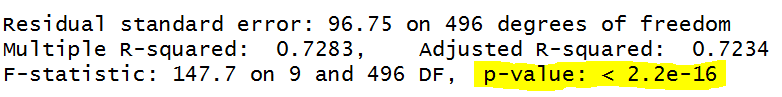
\includegraphics[width=4in]{r_sq_pval} \\
      \end{center}
      So we can reject the overall null hypothesis! \pause
      
      R-squared was already too big to suspect that it is zero and we already knew some predictors are statistically significant.
      
    \end{frame}  
   
   
    
    \begin{frame}[fragile]{How do we do with the predictions?}
      \fontsize{9}{9}\selectfont
      Let's plot the residuals, i.e., discrepancies between the predictions and the data.
      
\begin{knitrout}
\definecolor{shadecolor}{rgb}{0.137, 0.137, 0.137}\begin{kframe}
\begin{alltt}
\hlstd{> }\hlkwd{hist}\hlstd{(model}\hlopt{$}\hlstd{residuals,} \hlkwc{col}\hlstd{=}\hlstr{'green'}\hlstd{,}
\hlstd{+ }  \hlkwc{main}\hlstd{=}\hlstr{''}\hlstd{,} \hlkwc{xlab}\hlstd{=}\hlstr{'Residuals (in $1K)'}\hlstd{,} \hlkwc{ylab}\hlstd{=}\hlstr{'Frequency'}\hlstd{)}
\end{alltt}
\end{kframe}
\input{C:/temp/figures/unnamed-chunk-5-1.tikz}

\end{knitrout}
      
      
    \end{frame}  
    
    
    \begin{frame}[fragile]{How do we do with the predictions?}
      \fontsize{9}{9}\selectfont
      It looks like a normal distribution. Let's look at the mean of the residuals:
      
\begin{knitrout}
\definecolor{shadecolor}{rgb}{0.137, 0.137, 0.137}\begin{kframe}
\begin{alltt}
\hlstd{> }\hlkwd{mean}\hlstd{(model}\hlopt{$}\hlstd{residuals)}
\end{alltt}
\begin{verbatim}
[1] -2.028049e-15
\end{verbatim}
\end{kframe}
\end{knitrout}
      Virtually zero. 
      
      It will be always zero since we allow an intercept and minimize the sum of squared residuals.
      
      \bigskip
      
      What about the standard deviation?
\begin{knitrout}
\definecolor{shadecolor}{rgb}{0.137, 0.137, 0.137}\begin{kframe}
\begin{alltt}
\hlstd{> }\hlkwd{sd}\hlstd{(model}\hlopt{$}\hlstd{residuals)}
\end{alltt}
\begin{verbatim}
[1] 95.88111
\end{verbatim}
\end{kframe}
\end{knitrout}
      By the 2 standard deviation rule, we could estimate that 95\% of the time residuals are in [-\$192K, \$192K] range.
    \end{frame}  
   
    
    \begin{frame}[fragile]{How do we do with the predictions?}
      \fontsize{9}{9}\selectfont
      
      Can we obtain a \alert{similar} measure directly from the summary of the regression?
      
      \note{Emphasize that standard error and what we get with sd() is similar, but not exactly the same. 
           sd() estimates the population std dev, standard error is obtained by dividing SS by the num. deg. of freedom. } \pause
           
      It is the Residual standard error!
\begin{knitrout}
\definecolor{shadecolor}{rgb}{0.137, 0.137, 0.137}\begin{kframe}
\begin{alltt}
\hlstd{> }\hlkwd{summary}\hlstd{(model)}\hlopt{$}\hlstd{sigma}
\end{alltt}
\begin{verbatim}
[1] 96.74708
\end{verbatim}
\end{kframe}
\end{knitrout}
      \quad \pause
      \begin{center}
        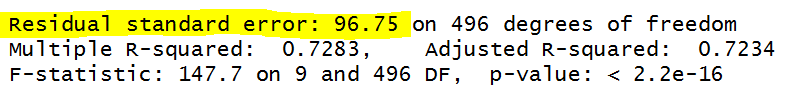
\includegraphics[width=4in]{std_err} \\
      \end{center}
      
    \end{frame}
    
    
    
    \begin{frame}{Again: regression assumptions}
      In multiple regression, we check on five things:
      \begin{enumerate}
        \item The residuals are independent.
        \item $Y$ is a linear function of $X$s (except for the errors).
        \item The residuals are normally distributed.
        \item The variance of $Y$ is the same for any value of $X$s (``homoscedasticity'').
        \item No multicollinearity between predictors.
      \end{enumerate}
    \end{frame}
    
    
    \begin{frame}[fragile]{Assumption 1: Independence}
      Independence: No correlation between residuals. \pause
    
      Difficult to verify this from plots, use: Durbin-Watson test. \pause
    
      \bigskip
    
      $H_0$: No correlation between residuals (i.e. independent).
    
      $H_1$: They are not independent \pause
    
      \bigskip
    
\begin{knitrout}
\definecolor{shadecolor}{rgb}{0.137, 0.137, 0.137}\begin{kframe}
\begin{alltt}
\hlstd{> }\hlkwd{durbinWatsonTest}\hlstd{(model)}
\end{alltt}
\begin{verbatim}
 lag Autocorrelation D-W Statistic p-value
   1       0.4918641      1.002805       0
 Alternative hypothesis: rho != 0
\end{verbatim}
\end{kframe}
\end{knitrout}
      \pause
    
      Oops... The model seems to have failed here. 
      
    \end{frame}
    

    
    
    
    \begin{frame}{Again: regression assumptions}
      In multiple regression, we check on five things:
      \begin{enumerate}
        \item The residuals are independent.
        \item $Y$ is a linear function of $X$s (except for the errors).
        \item The residuals are normally distributed.
        \item The variance of $Y$ is the same for any value of $X$s (``homoscedasticity'').
        \item No multicollinearity between predictors.
      \end{enumerate}
    \end{frame}
    
    
    
    \begin{frame}[fragile]{Assumption 2: Linearity}
    
\begin{knitrout}
\definecolor{shadecolor}{rgb}{0.137, 0.137, 0.137}\begin{kframe}
\begin{alltt}
\hlstd{> }\hlkwd{crPlots}\hlstd{(model,} \hlkwc{main}\hlstd{=}\hlstr{''}\hlstd{)}
\end{alltt}
\end{kframe}
\input{C:/temp/figures/unnamed-chunk-10-1.tikz}

\end{knitrout}
    \end{frame}   
    
    
    \begin{frame}{Again: regression assumptions}
      In multiple regression, we check on five things:
      \begin{enumerate}
        \item The residuals are independent.
        \item $Y$ is a linear function of $X$s (except for the errors).
        \item The residuals are normally distributed.
        \item The variance of $Y$ is the same for any value of $X$s (``homoscedasticity'').
        \item No multicollinearity between predictors.
      \end{enumerate}
    \end{frame}
    
    
    
    \begin{frame}[fragile]{Assumption 3: Normally distributed residuals}
    
\begin{knitrout}
\definecolor{shadecolor}{rgb}{0.137, 0.137, 0.137}\begin{kframe}
\begin{alltt}
\hlstd{> }\hlkwd{qqPlot}\hlstd{(model,} \hlkwc{col}\hlstd{=}\hlstr{'green'}\hlstd{)}
\end{alltt}
\end{kframe}
\input{C:/temp/figures/unnamed-chunk-11-1.tikz}

\end{knitrout}
    \end{frame}
    
    
    \begin{frame}{Again: regression assumptions}
      In multiple regression, we check on five things:
      \begin{enumerate}
        \item The residuals are independent.
        \item $Y$ is a linear function of $X$s (except for the errors).
        \item The residuals are normally distributed.
        \item The variance of $Y$ is the same for any value of $X$s (``homoscedasticity'').
        \item No multicollinearity between predictors.
      \end{enumerate}
    \end{frame}
    
    
    \begin{frame}[fragile]{Assumption 4: The variance of $Y$ is the same across}
    
\begin{knitrout}
\definecolor{shadecolor}{rgb}{0.137, 0.137, 0.137}\begin{kframe}
\begin{alltt}
\hlstd{> }\hlkwd{spreadLevelPlot}\hlstd{(model,} \hlkwc{col}\hlstd{=}\hlstr{'green'}\hlstd{,} \hlkwc{main}\hlstd{=}\hlstr{''}\hlstd{)}
\end{alltt}
\end{kframe}
\input{C:/temp/figures/unnamed-chunk-12-1.tikz}
\begin{kframe}\begin{verbatim}

Suggested power transformation:  0.8440952 
\end{verbatim}
\end{kframe}
\end{knitrout}
    \end{frame}
    
    
    \begin{frame}{Again: regression assumptions}
      In multiple regression, we check on five things:
      \begin{enumerate}
        \item The residuals are independent.
        \item $Y$ is a linear function of $X$s (except for the errors).
        \item The residuals are normally distributed.
        \item The variance of $Y$ is the same for any value of $X$s (``homoscedasticity'').
        \item No multicollinearity between predictors.
      \end{enumerate}
    \end{frame}
    
    
    \begin{frame}[fragile]{Assumption 5: No multicollinearity}
    
\begin{knitrout}
\definecolor{shadecolor}{rgb}{0.137, 0.137, 0.137}\begin{kframe}
\begin{alltt}
\hlstd{> }\hlkwd{sqrt}\hlstd{(}\hlkwd{vif}\hlstd{(model))}
\end{alltt}
\begin{verbatim}
   CRIME     ZONE      NOX     ROOM     DIST   RADIAL      TAX  PTRATIO 
1.326272 1.496362 1.932860 1.348359 1.851271 2.605272 2.684171 1.321139 
   LSTAT 
1.588188 
\end{verbatim}
\end{kframe}
\end{knitrout}
    \end{frame}
    
    
    \begin{frame}[fragile]{We have a model. What is next?}
    
      Make predictions
      
      Change one of the Xs by one unit
      
      Confidence Intervals: Mean Value and Single case
      
      
    
    \end{frame}
 
  \end{darkframes}

\end{document}
